\chapter{Diffusion Models}

\ca{Asegurarme la consistencia de notación con $\mathrm{x}$ y no $x$.}

\begin{figure}[ht]
    \centering
    \includegraphics[scale=0.22]{ch2-diffusion-models/fwd_noise.png}
    \captionsetup{width=\textwidth} % set the width of the caption
    \caption{Grogu (aka baby Yoda) through a forward process...\ca{Ver como mejorar estas imagen en resolución...}}
    \label{fig:fwd-process-grogu}
\end{figure}
  
In this chapter, we introduce the Diffusion Model, a family of generative models that have proven to be a valuable framework for novel image generation, text-to-image, text-to-video, and practical applications such as molecular graph modeling and medical image reconstruction \citep{sohldickstein2015deep, ramesh2021zeroshot,rombach2022highresolution,ho2020denoising,singer2022makeavideo,jing2023torsional,song2020denoising}. Proving to be a useful tool and keep this kind of model to be an active research line in the last few years \citep{yang2024diffusion}. \\

We will review the formulation proposed in the work titled \textit{Denoising Diffusion Probabilistic Models} \cite{ho2020denoising}, or DDPM for short. 
The primary motivation for basing the discussion of diffusion models on this work is to understand how the pretrained model that this work is based on was trained. In addition, it serves as a framework to understand subsequent improvements and enhancements without significant modifications to the primary ingredients of the recipe. Furthermore, it has a deep connection with theoretical work of score-based generative models \citep{song2020denoising} and Variational Autoencoders \citep{luo2022understanding}.

\section{Denoising Diffusion Probabilistic Models}

The key idea in denoising diffusion probabilistic models (DDPM) is to learn a mapping from a complex data distribution to a simple prior distribution, such as a Gaussian. This is achieved by successively corrupting the data with noise, transforming observations of the complex distribution into observations of the simple one. Concurrently, a model is trained to denoise the sequence of noisy observations and recover the original data.\\

Concretely, a forward process which starts from the raw image $\mathrm{x}_{0}$ (or whatever input) and creates a sequence of intermediate steps between $\mathrm{x}_{1}$ and $\mathrm{x}_{T-1}$, also known as latent states, which are noise perturbations in some degree of the original image's structure as shown in Figure~\ref{fig:fwd-process-grogu}. At the end of the sequence $T$---\textit{if the chain large is infinitely large}---the image is ultimately converting into an isotropic Gaussian noise $p(\mathrm{x}_{T})\sim \mathcal{N}(\mathrm{0}, \mathrm{I})$\footnote{Isotropic is a fancy word for ``equal shape'', and in this context means that the direction of the covariance matrix is all equal.}.\\

The authors model this forward process $q(\mathrm{x}_{1}\dots\mathrm{x}_{T}\mid\mathrm{x}_{0})$ as a Markov chain, and it is follow a normal distribution without learnable parameters (kernel). 
\begin{align}\label{eqn:forward-process}
q(\mathbf{x}_{1:T}\mid\mathrm{x}_0) &= \prod_{t=1}^{T}q(\mathrm{x}_t\mid\mathrm{x}_{t-1})
\\
q(\mathrm{x}_t\mid\mathrm{x}_{t-1}) &= \mathcal{N}(\mathrm{x}_t;\sqrt{1-\beta_{t}}~\mathrm{x}_{t-1},~ \beta_{t}\mathrm{I})
\end{align}
A deterministic noise scheduler is known beforehand and provides the
amount of noise $\beta_{t}$ for any timestep $t$ of the Markov chain to
generate $\mathrm{x}_{t}$ . How do we think about the latent space? The scale-location transformation\footnote{A quick recap about normal distributions, if $Z$ is a standard normal random variable and $X=\mu + \sigma Z$, then $X$ is a normal random variable with mean $\mu$ and variance $\sigma^2$, i.e. $X\sim\mathcal{N}(\mu, \sigma^2)$.} of $q(\mathrm{x}_{t}\mid\mathrm{x}_{t-1})\sim\mathcal{N}(\mathrm{x}_{t}; \sqrt{1-\beta_{t}} \mathrm{x}_{t-1}, \beta_{t}I)$ allows us to sample the \textcolor{orange}{current latent state $\mathrm{x}_{t}$ as a mixture} of the 
\textcolor{violet}{perturbation injected from noise} $\epsilon_{t-1}$ and \textcolor{teal}{the remaning structure
of the data} from the previous latent state $\mathrm{x}_{t-1}$.

%\textcolor{violet}{how much perturbation inject} from noise $\epsilon_{t-1}$, and \textcolor{teal}{the rest of what left of the image's structure} from the previous latent space $\mathrm{x}_{t-1}$:
\begin{equation}\label{eqn:scale-location-transformation}
    \textcolor{orange}{\mathrm{x}_{t}} = \textcolor{teal}{\sqrt{1-\beta_{t}}}~ \mathrm{x}_{t-1} + \textcolor{violet}{\sqrt{\beta_{t}}}~\mathrm{\epsilon}_{t-1}
\end{equation}
At the same time, there is a backward process---\textit{another Markov chain but in this case in the reverse timestep direction and with a learnable transition kernel}---model by $p_{\theta}(\mathrm{x}_{T:0})$. Specifically, 
the backward process takes the following form
\begin{align}\label{eqn:backward-process}
    p_{\theta}(\mathrm{x}_{T:0}) &= p(\mathrm{x}_{T})\prod_{t=1}^{T}p_{\theta}(\mathrm{x}_{t-1}\mid\mathrm{x}_{t})
    \\
    p_{\theta}(\mathrm{x}_{t-1}\mid\mathrm{x_{t}}) &= \mathcal{N}(\mathrm{x}_{t-1};~\mu_{\theta}(\mathrm{x}_{t}, t),~\Sigma_{\theta}(\mathrm{x}_{t}, t))
\end{align}
We know that $p(\mathrm{x}_{T})$ is a standard normal distribution when $\beta_{T}\approx 1$ in Eq.~\ref{eqn:scale-location-transformation}. Additionally, as we will see in the following sections, there are design options for learning 
the parameters of the kernel mentioned above. However, in most cases where the data distribution is complex, such as with images or audio, the kernel parameters are parameterized by deep neural networks.\\

\section{Recursive Reparameterization Trick}\label{sec:reparameterization-trick}

% https://stats.stackexchange.com/questions/199605/how-does-the-reparameterization-trick-for-vaes-work-and-why-is-it-important
% https://web.archive.org/web/20160418040123/http://dpkingma.com/wordpress/wp-content/uploads/2015/12/talk_nips_workshop_2015.pdf
The \textit{reparameterization trick} originally appears in the work that introduce the Variational Autoencoder (VAE) model \cite{kingma2013auto} and is also used in the diffusion framework with some modifications. The main goal in the VAE context is to remove the stochasticity of a node variable that depends on parameters from the distribution, \href{https://web.archive.org/web/20160418040123/http://dpkingma.com/wordpress/wp-content/uploads/2015/12/talk_nips_workshop_2015.pdf}{leaving the stochastic part as the noise instantiated in a separate node} (\ca{agregar diagrama de presentación Kignma? o reproducción de este?}). As simple as it appears, this trick makes it possible to create a computational graph to properly backpropagate and update the parameters during training. Nevertheless, in the diffusion context, we will
see that a \textit{recursive} application of the reparameterization trick achieve more than just enabling backpropagation. \\

Let $\alpha_{t}=1 - \beta_{t}$ and $\bar{\alpha}_{t}=\prod_{i=1}^{t}\alpha_{i}$. Now we proceed to unwind the $t$ index until $t=0$ in the sampling formula
that we can sample from any arbitrary normal distribution just scaling the
normal standard distribution $\sim \mathcal{N}(0, \sigma^2)$ accordingly its
parameters:
\begin{equation}\label{reparameterization-trick}
    \begin{split}
            \mathrm{x}_{t} & = \sqrt{\alpha_{t}}~\mathrm{x}_{t-1} + \sqrt{1-\alpha_{t}}~\epsilon_{t-1} \\
             & = \sqrt{\alpha_{t}}~(\sqrt{\alpha_{t-1}}~\mathrm{x}_{t-2} + \sqrt{1 - \alpha_{t-1}}~\epsilon_{t-2}) + \sqrt{1-\alpha_{t}}~\epsilon_{t-1} \\
             &= \sqrt{\alpha_{t}~\alpha_{t-1}}~\mathrm{x}_{t-2} + \textcolor{teal}{\sqrt{\alpha_{t} - \alpha_{t}~\alpha_{t-1}}~\epsilon_{t-2} + \sqrt{1-\alpha_{t}}~\epsilon_{t-1}} \\
             &= \sqrt{\alpha_{t}~\alpha_{t-1}}~\mathrm{x}_{t-2} + \textcolor{teal}{\sqrt{1 - \alpha_{t}~\alpha_{t-1}}~\bar{\epsilon}_{t-2}} \\
             &= \dots \\
             &= \sqrt{\alpha_{t}~\alpha_{t-1}\dots\alpha_{0}}~\mathrm{x}_{0} + \sqrt{1 - \alpha_{t}~\alpha_{t-1}\dots\alpha_{0}}~\bar{\epsilon}_{0} \\
             &= \sqrt{\prod_{i=1}^{t}\alpha_{i}}~\mathrm{x}_{0} + \sqrt{1 - \prod_{i=1}^{t}\alpha_{i}}~\bar{\epsilon}_{0} \\
             &= \sqrt{\bar{\alpha}_{t}}~\mathrm{x}_{0} + \sqrt{1 - \bar{\alpha}_
             {t}}~\bar{\epsilon}_{0} \\
            q(\mathrm{x}_{t}\mid \mathrm{x}_{0}) & = \mathcal{N}(\mathrm{x}_{t};\sqrt{\bar{\alpha}_{t}}~\mathrm{x}_{0}, (1-\bar{\alpha}_{t})\mathrm{I})
    \end{split}
\end{equation}
Technically, what happens in the above derivation is that the choice of a Gaussian transition kernel $q(\mathrm{x}_{t}\mid\mathrm{x}_{t-1})$ allows us to
\textcolor{teal}{group pairs of Gaussians into a single one, remaining a Gaussian distribution, by just summing up their means and variances}.  By repeteadly performing this trick, we end up marginilizing the joint distribution in Equation~\ref{eqn:forward-process} to obtain an analytical form of $q(\mathrm{x}_{t}\mid \mathrm{x}_{0})$ for all timesteps $t\in\{0, 1, \dots, T\}$, as shown in \shortcite{sohldickstein2015deep}. The remarkable consequence of having a closed form is the ability to sample from $\mathrm{x}_{0}\rightarrow \mathrm{x}_{t}$ without explicitly passing through intermediate steps $\mathrm{x}_{1}, \dots, \mathrm{x}_{t-1}$. Therefore, we can go from $\mathrm{x}_{0}$ to any arbitrary $t$ in just one evaluation---\textit{since $\bar{\alpha}$ is known in advance given the noise scheduler}---making the whole DDPM framework computationally feasible.

\section{Optimization}

\ca{\textbf{TODO:} partir directamente con la función de pérdida y especificando que en el paper de DDPM solo se parametriza el backward kernel para aprender la mediana. Especificmente, se aprende indirectamente a través de una reparametrización para aprender el ruido. La varianza es constante dependiente del tiempo y esta definiida por el noise scheduler.}

For training DDPM, the paper only uses the mean squared error (MSE) loss to optimize the backward kernel parameters. The MSE loss is defined as the expected value of the squared difference between the noise perturbation $\epsilon$ and the noise perturbation generated by the backward kernel $\epsilon_{\theta}$. The MSE loss is defined as follows: \\

The train objective defined in DDPM is the following loss, they choose to
paramterized the backward kernel only with the mean as a learnable parameter, 
and use a fixed time constant $\sigma_{t}^{2}=\sigma^{2}$ for all timesteps $t$:
\begin{equation}\label{eqn:ho-eq12}
    \mathbb{E}_{t\sim\mathcal{U}[1, T], \mathrm{x}_{0}\sim q(\mathrm{x}_{0}), \epsilon\sim\mathcal{N}(0, \mathrm{I}))} = \big[\lambda(t) ~ \|\epsilon - \epsilon_{\theta}(\mathrm{x}_{t}, t) \|^{2} \big]
\end{equation}
Where $\lambda(t)= \beta_{t}^{2} / 2\sigma_{t}^{2}\alpha_{t}(1-\bar{\alpha}_{t})$. Even it can simplify without any significant sample quality in...
\begin{equation}\label{eqn:ho-eq14}
    \mathbb{E}_{\mathrm{x}_{0}, \epsilon} \big[\| \epsilon - \epsilon_{\theta} ||^{2} \big]
\end{equation}
The simplified loss is just a mean squared error and we can train a DDPM
model using the algorithm XYZ.
\begin{figure}[ht]
    \begin{minipage}{0.45\textwidth}
    \begin{algorithm}[H]
        \caption{DDPM Training}
        \begin{algorithmic}
            \STATE \textbf{repeat}
            \STATE  ~~~~$\mathrm{x}_{0}\sim q(\mathrm{x_{0}})$
            \STATE  ~~~~$t\sim \mathcal{U}(1, T)$
            \STATE  ~~~~$\epsilon\sim \mathcal{N}(0, \mathrm{I})$
            \STATE  ~~~~Take gradient descent step on
            \STATE  $~~~~~~~~\nabla_{\theta}\|\epsilon - \epsilon_{\theta}(\sqrt{\bar{\alpha}_{t}}\mathrm{x}_{0} + \sqrt{1-\bar{\alpha}_{t}}\epsilon, t) \|^{2}$
            \STATE \textbf{until} converged
        \end{algorithmic}
    \end{algorithm}
    \end{minipage}
    \hspace{0.25cm}
    %\hfill
    \begin{minipage}{0.45\textwidth}
    \begin{algorithm}[H]
        \caption{DDPM Sampling}
        \begin{algorithmic}
        \STATE  $\mathrm{x}_{T}\sim\mathcal{N}(\mathrm{0}, \mathrm{I})$
        \FOR{$t=T, \dots, 1$}
            \STATE $\mathrm{z}\sim\mathcal{N}(0, \mathrm{I})$
            \STATE $\mathrm{x}_{t-1}=\frac{1}{\sqrt{\alpha_{t}}} \bigg(\mathrm{x}_{t} - \frac{1-\alpha_{t}}{\sqrt{1-\bar{\alpha}_{t}}}\epsilon_{\theta}(\mathrm{x}_{t}, t)\bigg) + \sigma_{t}\mathrm{z}$
        \ENDFOR
        \STATE \textbf{return} $\mathrm{x}_{0}$
        \end{algorithmic}
    \end{algorithm}
    \end{minipage}
    \end{figure}

\ca{Para entender la reparametrización del backward kernel para usar un epsilon}.\\

\ca{\textbf{Importante:} la reparametrización que aparece en el algoritmo de
sampling, la derivación para llegar a esta se encuentra en \href{https://lilianweng.github.io/posts/2021-07-11-diffusion-models/}{post de difusion de Lilian Weng} } \\

In the next sections we will justify the use of the above loss function and the training algorithm in the context of the Variational Lower Bound (VLB).

\subsection{Variational Lower Bound}\label{sec:variational-lower-bound}

    %https://chrisorm.github.io/VI-ELBO.html
    %esto se puede derivar desde la divergencia de Kullback-Leibler
    % o usando Jensen Inequality. En paper summary se ocupa KL, se podría
    % mostrar esa conciliaición...

    DDPM are training by optimizing the Variational Lower Bound (VLB)
    on the negative log-likelihood.\ca{Referencia al apendica A del paper de DDPM.}
    \begin{equation}\label{eqn:ELBO1}
    \begin{split} 
    -\log p_{\theta}(\mathrm{x}_{0}) &= -\log\int p_{\theta}(\mathrm{x}_{0:T}) d\mathrm{x}_{1:T} \\
    &= -\log \int \frac{p_{\theta}(\mathrm{x}_{0:T})q(\mathrm{x}_{1:T}\mid\mathrm{x}_{0})}{q(\mathrm{x}_{1:T}\mid\mathrm{x}_{0})}d\mathrm{x}_{1:T} \\
    &= - \log \mathbb{E}_{q(\mathrm{x}_{1:T}\mid\mathrm{x}_0)} \bigg[\frac{p_{\theta}(\mathrm{x}_{0:T})}{q(\mathrm{x}_{1:T}\mid\mathrm{x}_{0})} \bigg] \\
    % -\log p_{\theta}(\mathrm{x}_{0}) 
    & \leq \mathbb{E}_{q(\mathrm{x}_{1:T}\mid\mathrm{x}_{0})}\bigg[-\log \frac{p_{\theta}(\mathrm{x}_{0:T})}{q(\mathrm{x}_{1:T}\mid\mathrm{x}_{0})}\bigg] \\
    &\leq \mathbb{E}_{q(\mathrm{x}_{1:T}\mid\mathrm{x}_{0})}\bigg[-\log p(\mathrm{x}_{T}) - \sum_{t\geq 1}^{T} \log\frac{p_{\theta}(\mathrm{x}_{t-1}\mid\mathrm{x}_{t})}{q(\mathrm{x}_{t}\mid\mathrm{x}_{t-1})} \bigg] \\
    L &:= \mathbb{E}_{q(\mathrm{x}_{1:T}\mid\mathrm{x}_{0})}\bigg[-\log p(\mathrm{x}_{T}) - \sum_{t>1}^{T} \log \frac{p_{\theta}(\mathrm{x}_{t-1}\mid\mathrm{x}_{t})}{q(\mathrm{x}_{t}\mid\mathrm{x}_{t-1})}-\log\frac{p_{\theta}(\mathrm{x}_{0}\mid\mathrm{x}_{1})}{q(\mathrm{x}_{1}\mid\mathrm{x}_{0})}\bigg]
    \end{split}
    \end{equation}
    \ca{Actualizar párrafo, ahora Jensen inequality se aplica en el paso 3...}
    The first relationship in \ref{eqn:ELBO1} can be justified by the Jensen's inequality, and the second relationship is a direct consequence of the Markov property in both the forward and backward processes. Also, notice that we decouple the last term $\mathrm{x}_{T}$ from $p_{\theta}(\mathrm{x}_{0:T})$ because,
    for a sufficiently large sequence $T\gg$, we know that we will get a final state described by $\mathcal{N}(0, \sigma^2\mathrm{I})$. Therefore, we keep it separate in the same way as the first transition step $\mathrm{x}_{0}\mid\mathrm{x_{1}}$ and $\mathrm{x}_1\mid\mathrm{x}_0$ that involves the raw data $\mathrm{x}_{0}$ in each process.\\
    
    We obtain the training objective from the VLB following the derivations in \cite{sohldickstein2015deep} and \cite{ho2020denoising}: \ca{cambiar todos los $x$ a $\mathrm{x}$ y usar mid en vez de la línea vertical |}
    For space constraint, we are referring to $\mathbb{E}_{q(\mathrm{x}_{1:T}\mid\mathrm{x}_{0})}$ when it appears $\mathbb{E}_{q}$.
    \begin{equation}\label{eqn:ELBO2}
    \begin{split}
     L_{\text{\scriptsize{\text{VLB}}}} & = \mathbb{E}_{q}\bigg[-\log p(\mathrm{x}_{T}) - \sum_{t>1}^{T} \log \frac{p_{\theta}(\mathrm{x}_{t-1}\mid\mathrm{x}_{t})}{q(\mathrm{x}_{t}\mid\mathrm{x}_{t-1})}-\log\frac{p_{\theta}(\mathrm{x}_{0}\mid\mathrm{x}_{1})}{q(\mathrm{x}_{1}\mid\mathrm{x}_{0})}\bigg] \\
    & = \mathbb{E}_{q}\bigg[-\log p(\mathrm{x}_{T}) - \sum_{t>1}^{T} \log \frac{p_{\theta}(\mathrm{x}_{t-1}\mid\mathrm{x}_{t})}{\textcolor{teal}{q(\mathrm{x}_{t-1}\mid\mathrm{x}_{t},~\mathrm{x}_{0})}}\frac{\textcolor{lightgray}{q(\mathrm{x}_{t-1}\mid\mathrm{x}_{0})}}{\textcolor{violet}{q(\mathrm{x}_{t}\mid\mathrm{x}_{0})}}-\log\frac{p_{\theta}(\mathrm{x}_{0}\mid\mathrm{x}_{1})}{q(\mathrm{x}_{1}\mid\mathrm{x}_{0})}\bigg] \\
    & = \mathbb{E}_{q}\bigg[-\log p(\mathrm{x}_{T}) - \sum_{t>1}^{T} \log \frac{p_{\theta}(\mathrm{x}_{t-1}\mid\mathrm{x}_{t})}{\textcolor{teal}{q(\mathrm{x}_{t-1}\mid\mathrm{x}_{t},~\mathrm{x}_{0})}} -\sum_{t>1}^{T}\log \frac{\textcolor{lightgray}{q(\mathrm{x}_{t-1}\mid\mathrm{x}_{0})}}{\textcolor{violet}{q(\mathrm{x}_{t}\mid\mathrm{x}_{0})}}-\log\frac{p_{\theta}(\mathrm{x}_{0}\mid\mathrm{x}_{1})}{q(\mathrm{x}_{1}\mid\mathrm{x}_{0})}\bigg] \\
    & = \mathbb{E}_{q}\bigg[-\log p(\mathrm{x}_{T}) - \sum_{t>1}^{T} \log \frac{p_{\theta}(\mathrm{x}_{t-1}\mid\mathrm{x}_{t})}{\textcolor{teal}{q(\mathrm{x}_{t-1}\mid\mathrm{x}_{t}, \mathrm{x}_{0})}}- \log\frac{\textcolor{orange}{q(\mathrm{x}_{1}\mid\mathrm{x}_{0})}}{\textcolor{violet}{q(\mathrm{x}_{T}\mid\mathrm{x}_{0})}} -\log\frac{p_{\theta}(\mathrm{x}_{0}\mid\mathrm{x}_{1})}{q(\mathrm{x}_{1}\mid\mathrm{x}_{0})}\bigg] \\
    & = \mathbb{E}_{q}\bigg[-\log p(\mathrm{x}_{T}) - \sum_{t>1}^{T} \log \frac{p_{\theta}(\mathrm{x}_{t-1}\mid\mathrm{x}_{t})}{\textcolor{teal}{q(\mathrm{x}_{t-1}\mid\mathrm{x}_{t}, \mathrm{x}_{0})}}- \log\textcolor{orange}{q(\mathrm{x}_{1}\mid\mathrm{x}_{0})} + \log \textcolor{violet}{q(\mathrm{x}_{T}\mid\mathrm{x}_{0})} -\log\frac{p_{\theta}(\mathrm{x}_{0}\mid\mathrm{x}_{1})}{q(\mathrm{x}_{1}\mid\mathrm{x}_{0})}\bigg] \\
    & = \mathbb{E}_{q}\bigg[-\big(\log p(\mathrm{x}_{T}) - \log \textcolor{violet}{q(\mathrm{x}_{T}\mid\mathrm{x}_{0})}\big) - \sum_{t>1}^{T} \log \frac{p_{\theta}(\mathrm{x}_{t-1}\mid\mathrm{x}_{t})}{\textcolor{teal}{q(\mathrm{x}_{t-1}\mid\mathrm{x}_{t}, \mathrm{x}_{0})}} - \big( \log\textcolor{orange}{q(\mathrm{x}_{1}\mid\mathrm{x}_{0})}  +\log\frac{p_{\theta}(\mathrm{x}_{0}\mid\mathrm{x}_{1})}{q(x_{1}\mid\mathrm{x}_{0})}\big)\bigg]  \\ 
    & = \mathbb{E}_{q}\bigg[-\log \frac{p(\mathrm{x}_{T})}{\textcolor{violet}{q(\mathrm{x}_{T}\mid\mathrm{x}_{0})}} - \sum_{t>1}^{T} \log \frac{p_{\theta}(\mathrm{x}_{t-1}\mid\mathrm{x}_{t})}{\textcolor{teal}{q(\mathrm{x}_{t-1}\mid\mathrm{x}_{t}, \mathrm{x}_{0})}} -  \log p_{\theta}(\mathrm{x}_{0}\mid\mathrm{x}_{1})\bigg]  \\
    & = \mathbb{E}_{q(\mathrm{x}_{1:T}\mid\mathrm{x}_{0})}\bigg[\underbrace{D_{\text{\scriptsize{KL}}}\big(\textcolor{violet}{q(\mathrm{x}_{T}\mid\mathrm{x}_{0})} ||~p(\mathrm{x}_{T}) \big)}_{L_{T}} + \sum_{t>1}^{T} \underbrace{D_{\text{\scriptsize{KL}}}\big( \textcolor{teal}{q(\mathrm{x}_{t-1}\mid\mathrm{x}_{t}, \mathrm{x}_{0})}||~p_{\theta}(\mathrm{x}_{t-1}\mid\mathrm{x}_{t}) \big)}_{L_{t-1}} -  \underbrace{\log p_{\theta}(\mathrm{x}_{0}\mid\mathrm{x}_{1})}_{L_{0}} \bigg]
    \end{split}
    \end{equation}

    \begin{enumerate}
        \item We isolated $\log q(\mathrm{x}_{t}\mid\mathrm{x}_{0})$ with $\log p(\mathrm{x}_{T})$ because both are invariant by the learning process.
        \item We reverse by Bayes theorem $q(\mathrm{x}_{t}\mid\mathrm{x}_{t-1})$ by $q(\mathrm{x}_{t-1}\mid\mathrm{x}_{t}, \mathrm{x}_{0})$ without affecting the markov property \ca{revisar vericidad de esto...}.
        \item The first both terms in Eq.~\ref{eqn:ELBO2} appears by the Kullback-Leibler divergence definition. 
    \end{enumerate}
    

    In summary, the variational lower bound loss is a sum of terms that arise from the reverse diffusion process $L_{\text{\scriptsize{\text{VLB}}}}=L_{T} + L_{T-1} + \dots + L_{0}$. The last term $L_{T}$ can be discard because
    is constant given thatt $q$ has not learnable parameters and $\mathrm{x}_{T}$ is a standard normal distribution. The remaining terms are the denoising matching terms that are the most important in the loss function because they have the most number of terms.\\

\subsection{Denoising Matching Term}
\begin{figure}[t]
  \centering
  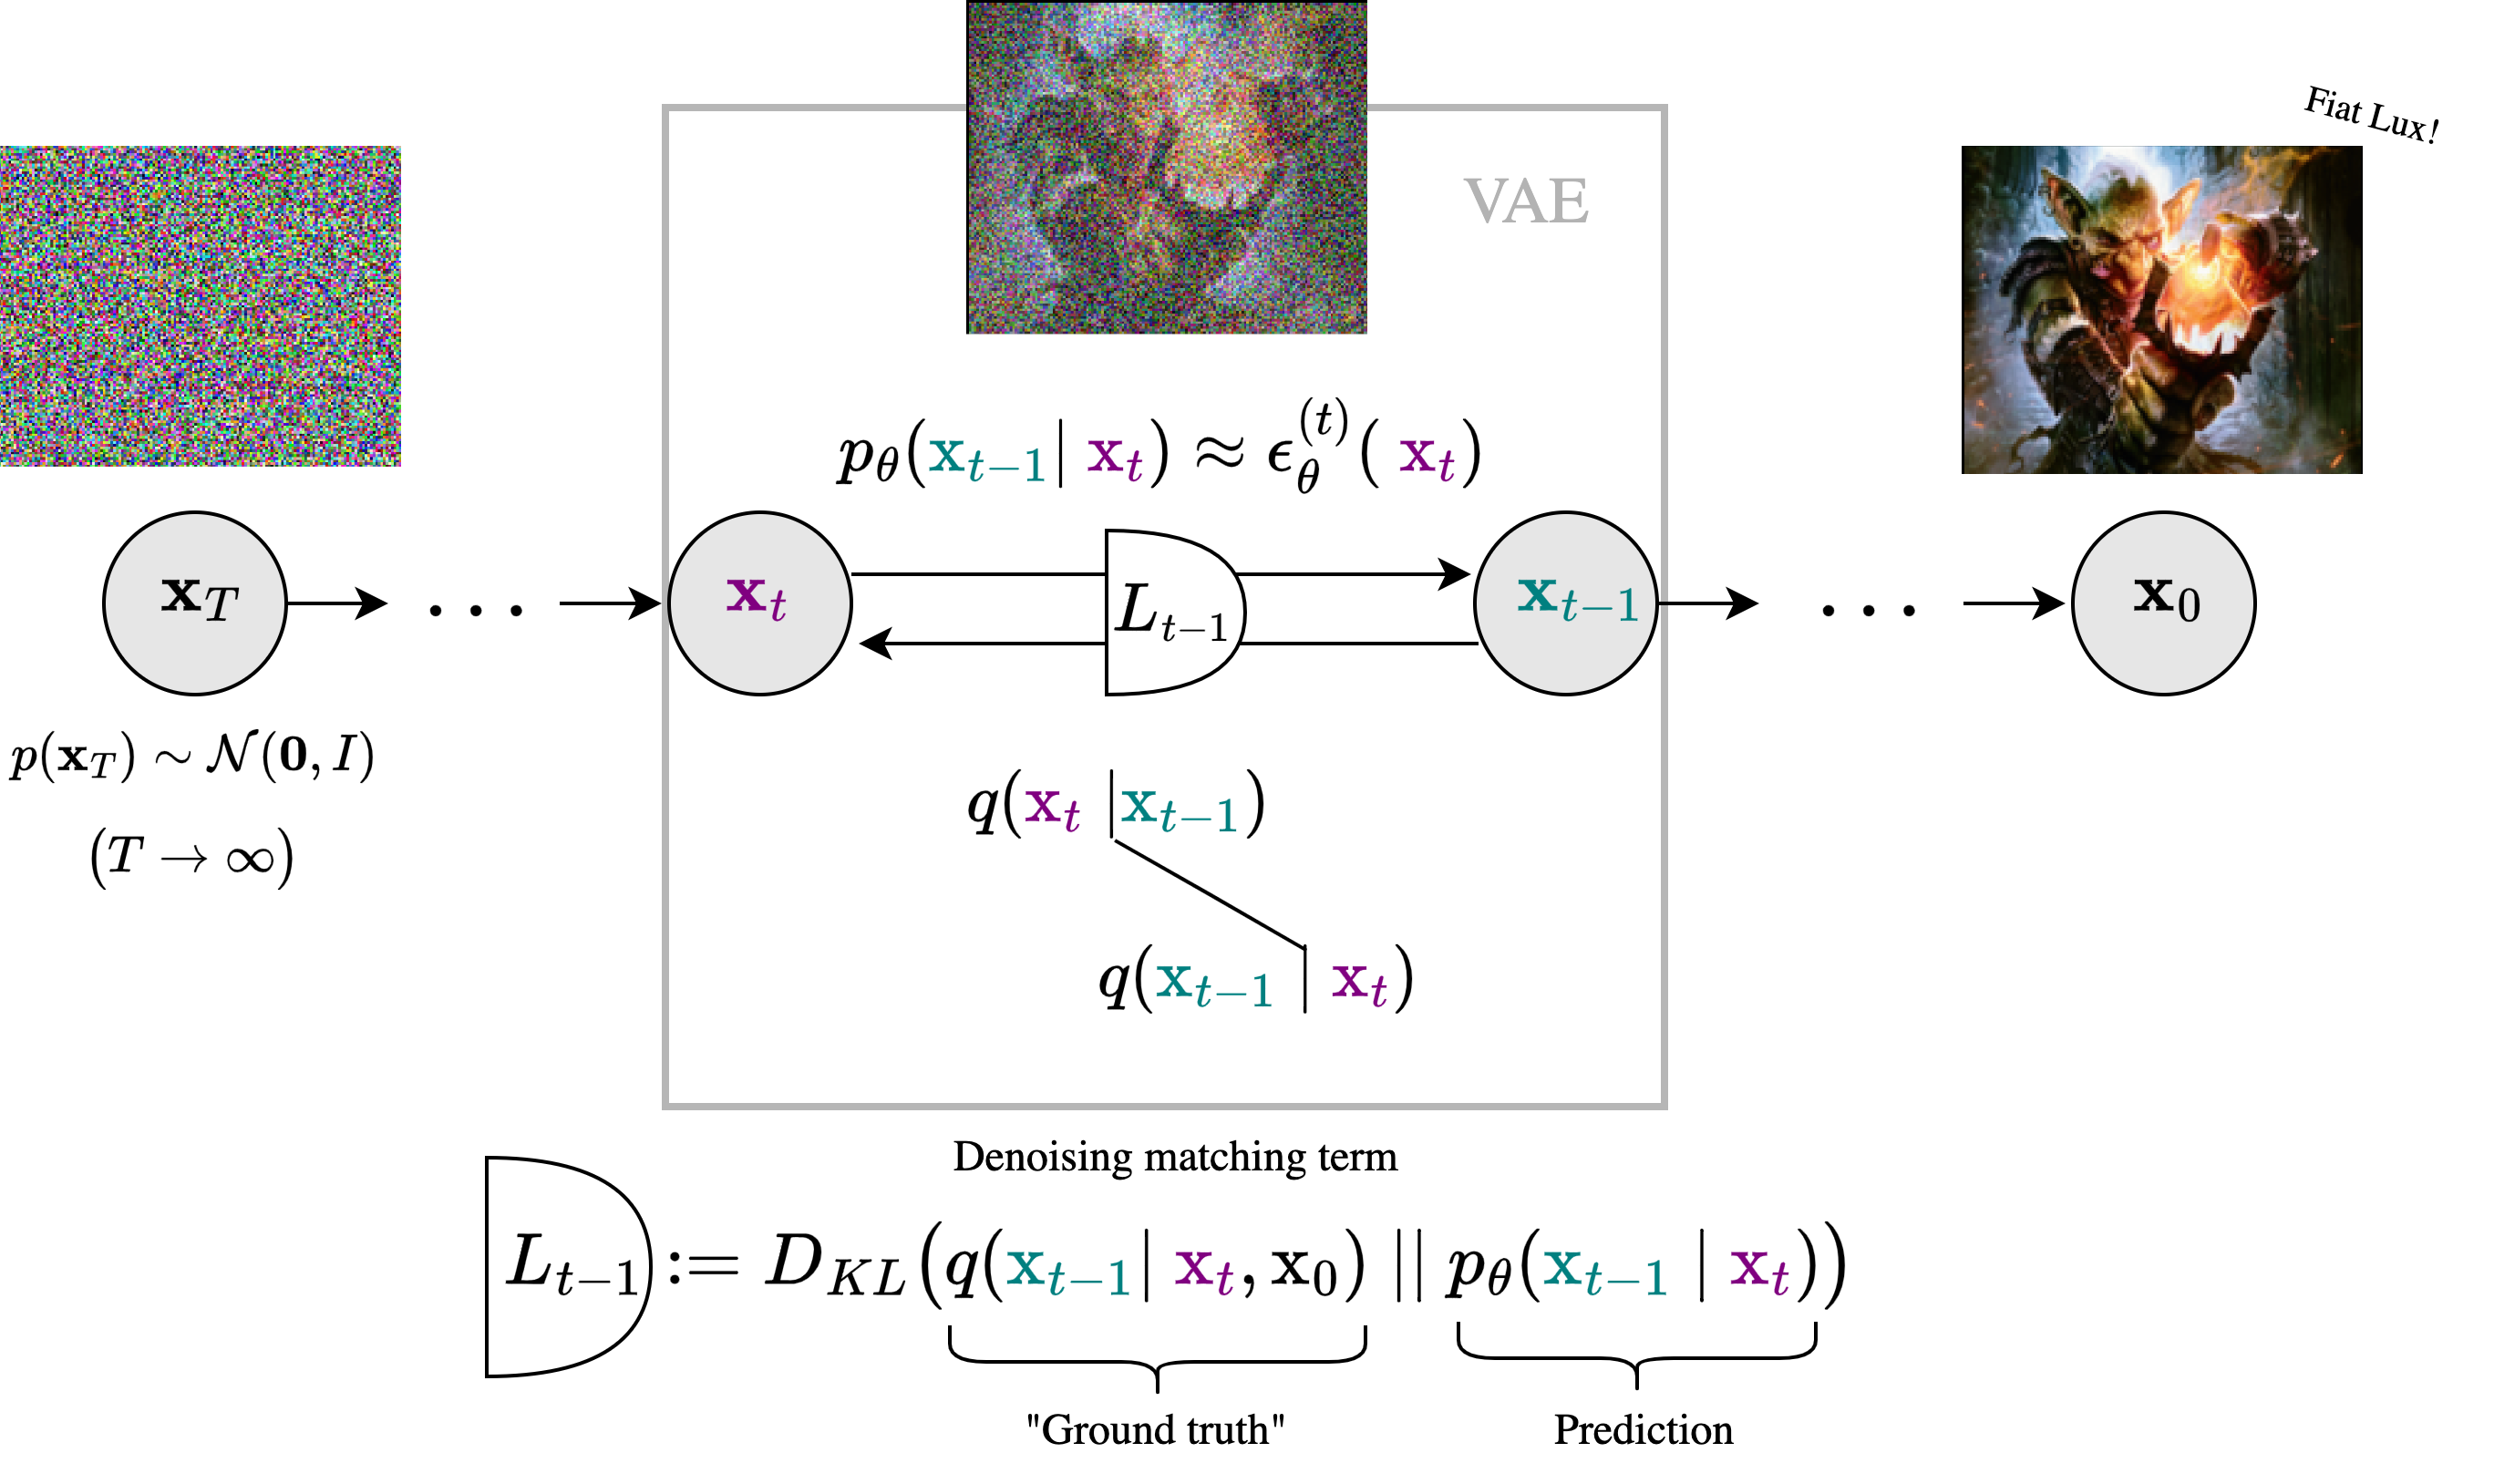
\includegraphics[scale=0.8]{ch2-diffusion-models/DDPM-HMVAE-simple.png}
  \captionsetup{width=\textwidth} % set the width of the caption
  \caption{\textbf{Denoising matching term in action.} $\mathrm{x}_{T}$ is a pure Gaussian noise. In the middle square, it highlights the transition from a noisy intermediate state to a less noisy one; the denoising matching term forces $p_{\theta}$ to be similar to the posterior forward kernel $q(\mathrm{x}_{t-1}\mid \mathrm{x}_{t})$. $\mathrm{x}_{0}$ the input image during training or the final sample at inference mode. \ca{Simplicar este caption esta muy verboso.}}
  \label{fig:ddpm-denoising-term}
\end{figure}
The model goal is to reduce the discrepancy measured by the Kullback-Leibler divergence between the posterior of the encoder, which tell us how to remove the real noise, and the decoder, which predicts to ``reverse'' the processes and has learnable parameters $(\theta)$. Therefore, the loss constitutes a sum of denoising matching terms across the diffusion sequence as it show in Figure~\ref{fig:ddpm-denoising-term}. \\

However, the problem is that reverse the diffusion process $q(\mathrm{x}_{t-1}\mid\mathrm{x}_{t})$ is intractable because requires the entire dataset to compute it, but we can conditioning on $\mathrm{x}_{0}$ to make it tractable and get the following expression (Lilian Weng \citep{weng2021diffusion}):
\begin{align}\label{eqn:reverse-forward-process}
    q(\mathrm{x}_{t-1}\mid\mathrm{x}_{t}, \mathrm{x}_{0}) &= \mathcal{N}(\mathrm{x}_{t-1};~\tilde{\mu}(\mathrm{x}_{t}, \mathrm{x}_{0}, t), \tilde{\beta}_{t}I) \\
    \tilde{\mu}(\mathrm{x}_{t}, t) &= \frac{1}{\sqrt{\alpha_{t}}}\bigg(\mathrm{x}_{t} - \frac{1 - \alpha_{t}}{\sqrt{1-\bar{\alpha}_{t}}} \epsilon_{t} \bigg) 
    % \\ \tilde{\beta}_{t} &= x
\end{align}
Another important aspect is the parameterization of $p_{\theta}$ we can predict directly the latent state $\mathrm{x}_{t-1}$, or indirectly by predicting the noise perturbation $\epsilon_{\theta}$ and then apply the reparameterization trick to get the latent state, given that $\mathrm{x}_{t}$ is known. Moreover,
in Ho et al \cite{ho2020denoising} they use only the mean as a learnable parameter and the variance is set as $\Sigma_{\theta}(\mathrm{x}_{t}, t)=\sigma_{t}^2I$, a time dependent constant such as $\sigma_{t}^{2}=\beta_{t}$ or $\sigma_{t}^{2}=\tilde{\beta}_{t}$.
\begin{align}\label{eqn:backward-noise-reparameterization}
    \mu_{\theta}(\mathrm{x}_{t}, t) &= \frac{1}{\sqrt{\alpha_{t}}}\big(\mathrm{x}_{t} - \frac{1-\alpha_{t}}{\sqrt{1-\bar{\alpha}_{t}}}\epsilon_{\theta}(\mathrm{x}_{t}, t)\big) \\
    \mathrm{x}_{t-1} &= \mathcal{N}\big(\mathrm{x}_{t-1}; \frac{1}{\sqrt{\alpha_{t}}}\big(\mathrm{x}_{t} - \frac{1-\alpha_{t}}{\sqrt{1-\bar{\alpha}_{t}}}\epsilon_{\theta}(\mathrm{x}_{t}, t)\big), \Sigma_{\theta}(\mathrm{x}_{t}, t)\big)
\end{align}

Backward parametrerization Ho. et al just use the mean as a learnable parameter, and the variance is fixed and time-depends on the noise scheduler, 
$\Sigma_{\theta}(\mathrm{x}_{t}, t) = \sigma_{t}^{2}I$:
\begin{align}\label{eqn:backward-process-fix-variance}
    p_{\theta}(\mathrm{x}_{t-1}\mid\mathrm{x_{t}}) &= \mathcal{N}(\mathrm{x}_{t-1};~\mu_{\theta}(\mathrm{x}_{t}, t), \sigma_{t}^{2}I)
\end{align}
Therefore, we have everything to expand the denoising matching term $L_t$ with $1\leq t < T$ terms:

\ca{Además, emerge de la definición de KL de sumatorias entre dos gaussiano un MSE.}



We can think of the above formulation as a hierarchical variational autoencoder that satisfies some properties as it is specified in \citep{luo2022understanding}. \ca{Conexión con VAE en Luo} As you can see in Figure~\ref{fig:ddpm-denoising-term}, the denoising matching term within the gray square remarks the VAE loss term. 


\subsection{Sampling}

\ca{Describir el algoritmo de sampling brevemente...}.

\subsection{Score-based generative models}

\textbf{TODO:} Explain the connection between score-based generative models and the DDPM.\\

Learning $\epsilon_{\theta}$ is equivalent to perturb the data distribution $p(x)$ in the direction of the score function $\nabla_{x}\log p(x)$, which is the gradient of the log-likelihood. This is a key idea in score-based generative models, where the model is trained to denoise the data by following the gradient of the log-likelihood.\\

Stein no sé cuanto...

    
\section{Condition the model}

\ca{Acá se salta a formulación score bared de la nada, ver como introducir antes...}

So far, we know how to learn indirectly the unconditional probability distribution $p(x)$ via the score function $\nabla_{x}\log p(x)$, but what can we do to condition $x$ given a signal $y$, such as a text prompt, another image, or an audio?\\

By Bayes' theorem, log operations, and taking the gradient w.r.t. x we got:

    \begin{equation}
         \begin{split}
            p(x \mid y) &= \frac{p(y \mid x) \cdot p(x)}{p(y)}\\
            \implies \log p(x \mid y) &= \log p(y \mid x) + \log p(x) - \log p(y) \\
            \implies \nabla_x \log p(x \mid y) &= \nabla_x \log p(y \mid x) + \nabla_x \log p(x) ,
        \end{split}
    \end{equation}
    

    \textbf{TODO:} Review and cite the following \href{https://sander.ai/2023/08/28/geometry.html}{blog posts} \cite{dieleman2022guidance} and \cite{dieleman2023geometry} about guidance.

\subsection{Classifier Guidance}

    Once a diffusion model is trained, during the sampling
    process (aka denoising Gaussian noise), we can attach
    a cost function that "guides" the denoising process toward
    some desired condition, such as colour or text embedding from a prompt that matches a text caption, gets by the image at each denoising step.\\ Introduce in \cite{nichol2021glide}.

    \textbf{TODO:} Mention and explain the Relevant work in the last part of this work \cite{Dhariwal2021DiffusionMB}.\\     

    \textbf{TODO:} Create a diagram to explain the classifier guidance. It could be used for text prompt guidance using CLIP.\\ \ca{Lo importante es mencionar como usar el espacio de embedding conjunto de CLIP en los modelos text-to-image para guairlos...}.

\begin{figure}[ht]
    \centering
    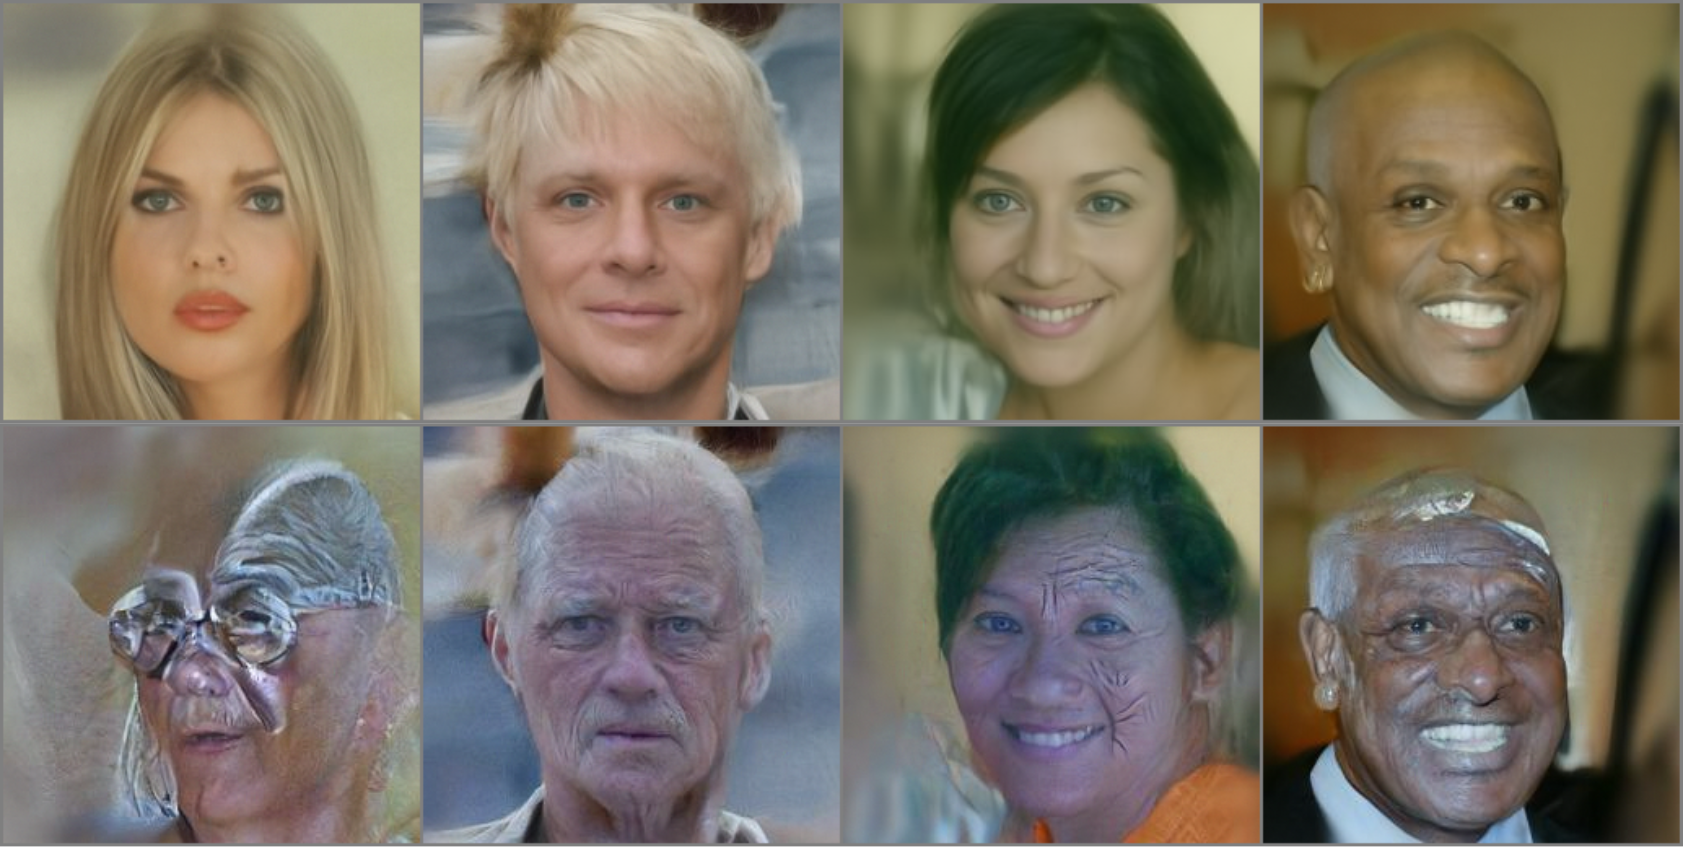
\includegraphics[scale=0.95]{ch2-diffusion-models/clip-guidance-experiment.png}
    \captionsetup{width=\textwidth} % set the width of the caption
    \caption{\textbf{CLIP classifier guidance.} Using the following prompt \texttt{old, senior, oldster, elderly, golden-ager} to denoise the noise seed that generate the four above images an update the model parameters in
    the direction of the prompt.}
    \label{fig:clip-guidance-old-experiment}
  \end{figure}

\begin{figure}[ht]
    \centering
    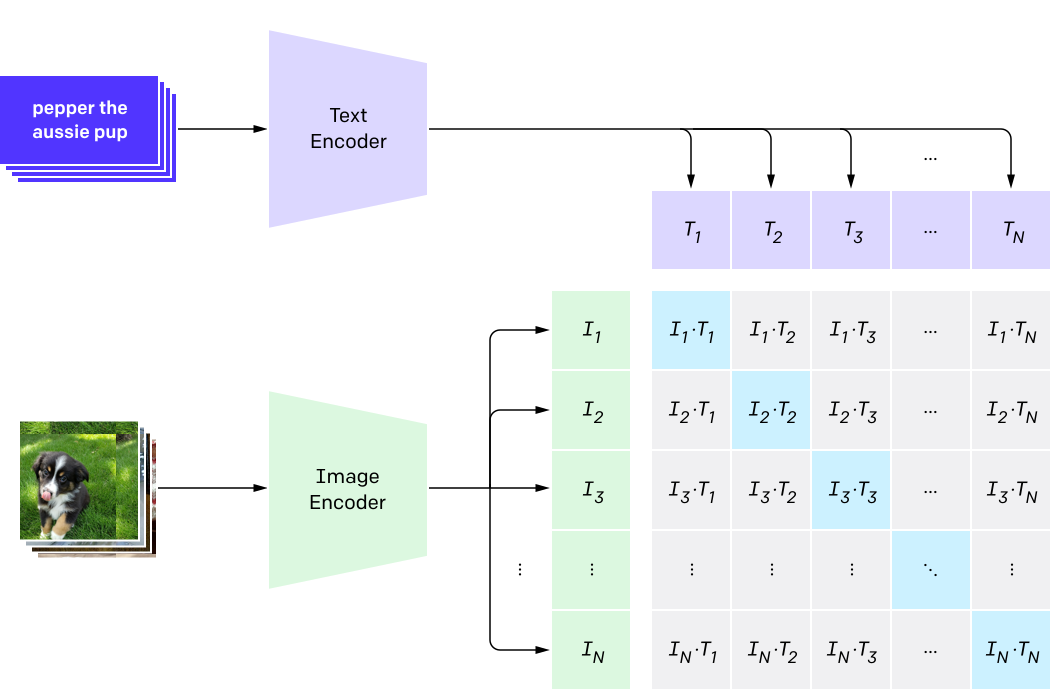
\includegraphics[scale=0.5]{ch2-diffusion-models/clip-overview-a.png}
    \captionsetup{width=\textwidth} % set the width of the caption
    %\caption{\textbf{CLIP overview.} Text-to-image joint embedding space. \textbf{Source:} Alec Radford, Jong Wook Kim, Chris Hallacy, Aditya Ramesh, Gabriel Goh, Sandhini Agarwal, Girish Sastry, Amanda Askell, Pamela Mishkin, Jack Clark, Gretchen Krueger, \& Ilya Sutskever. (2021). Learning Transferable Visual Models From Natural Language Supervision.}
    \caption{\textbf{CLIP overview.} Text-to-image joint embedding space. \textbf{Source:} Learning Transferable Visual Models From Natural Language Supervision \citep{radford2021learning}.}
    \label{fig:clip-overview}
  \end{figure}

    
\subsection{Classifier Free Guidance (CFG)}

    \textbf{TODO:} A good blog post that explains classifier guidance is \cite{dieleman2022guidance}. \\


\section{Enhancements \& Improvements}

Despite the progress in conditioning the model, there are...\\

A direct improvement to the DDPM was made in \cite{nichol2021improved}, in which they learn not only $\mu$ but also the variance $\sigma^{2}$ of the reverse process. This directly improves the likelihood estimation achieved by the model. \\

\begin{figure}[ht]
    \centering
    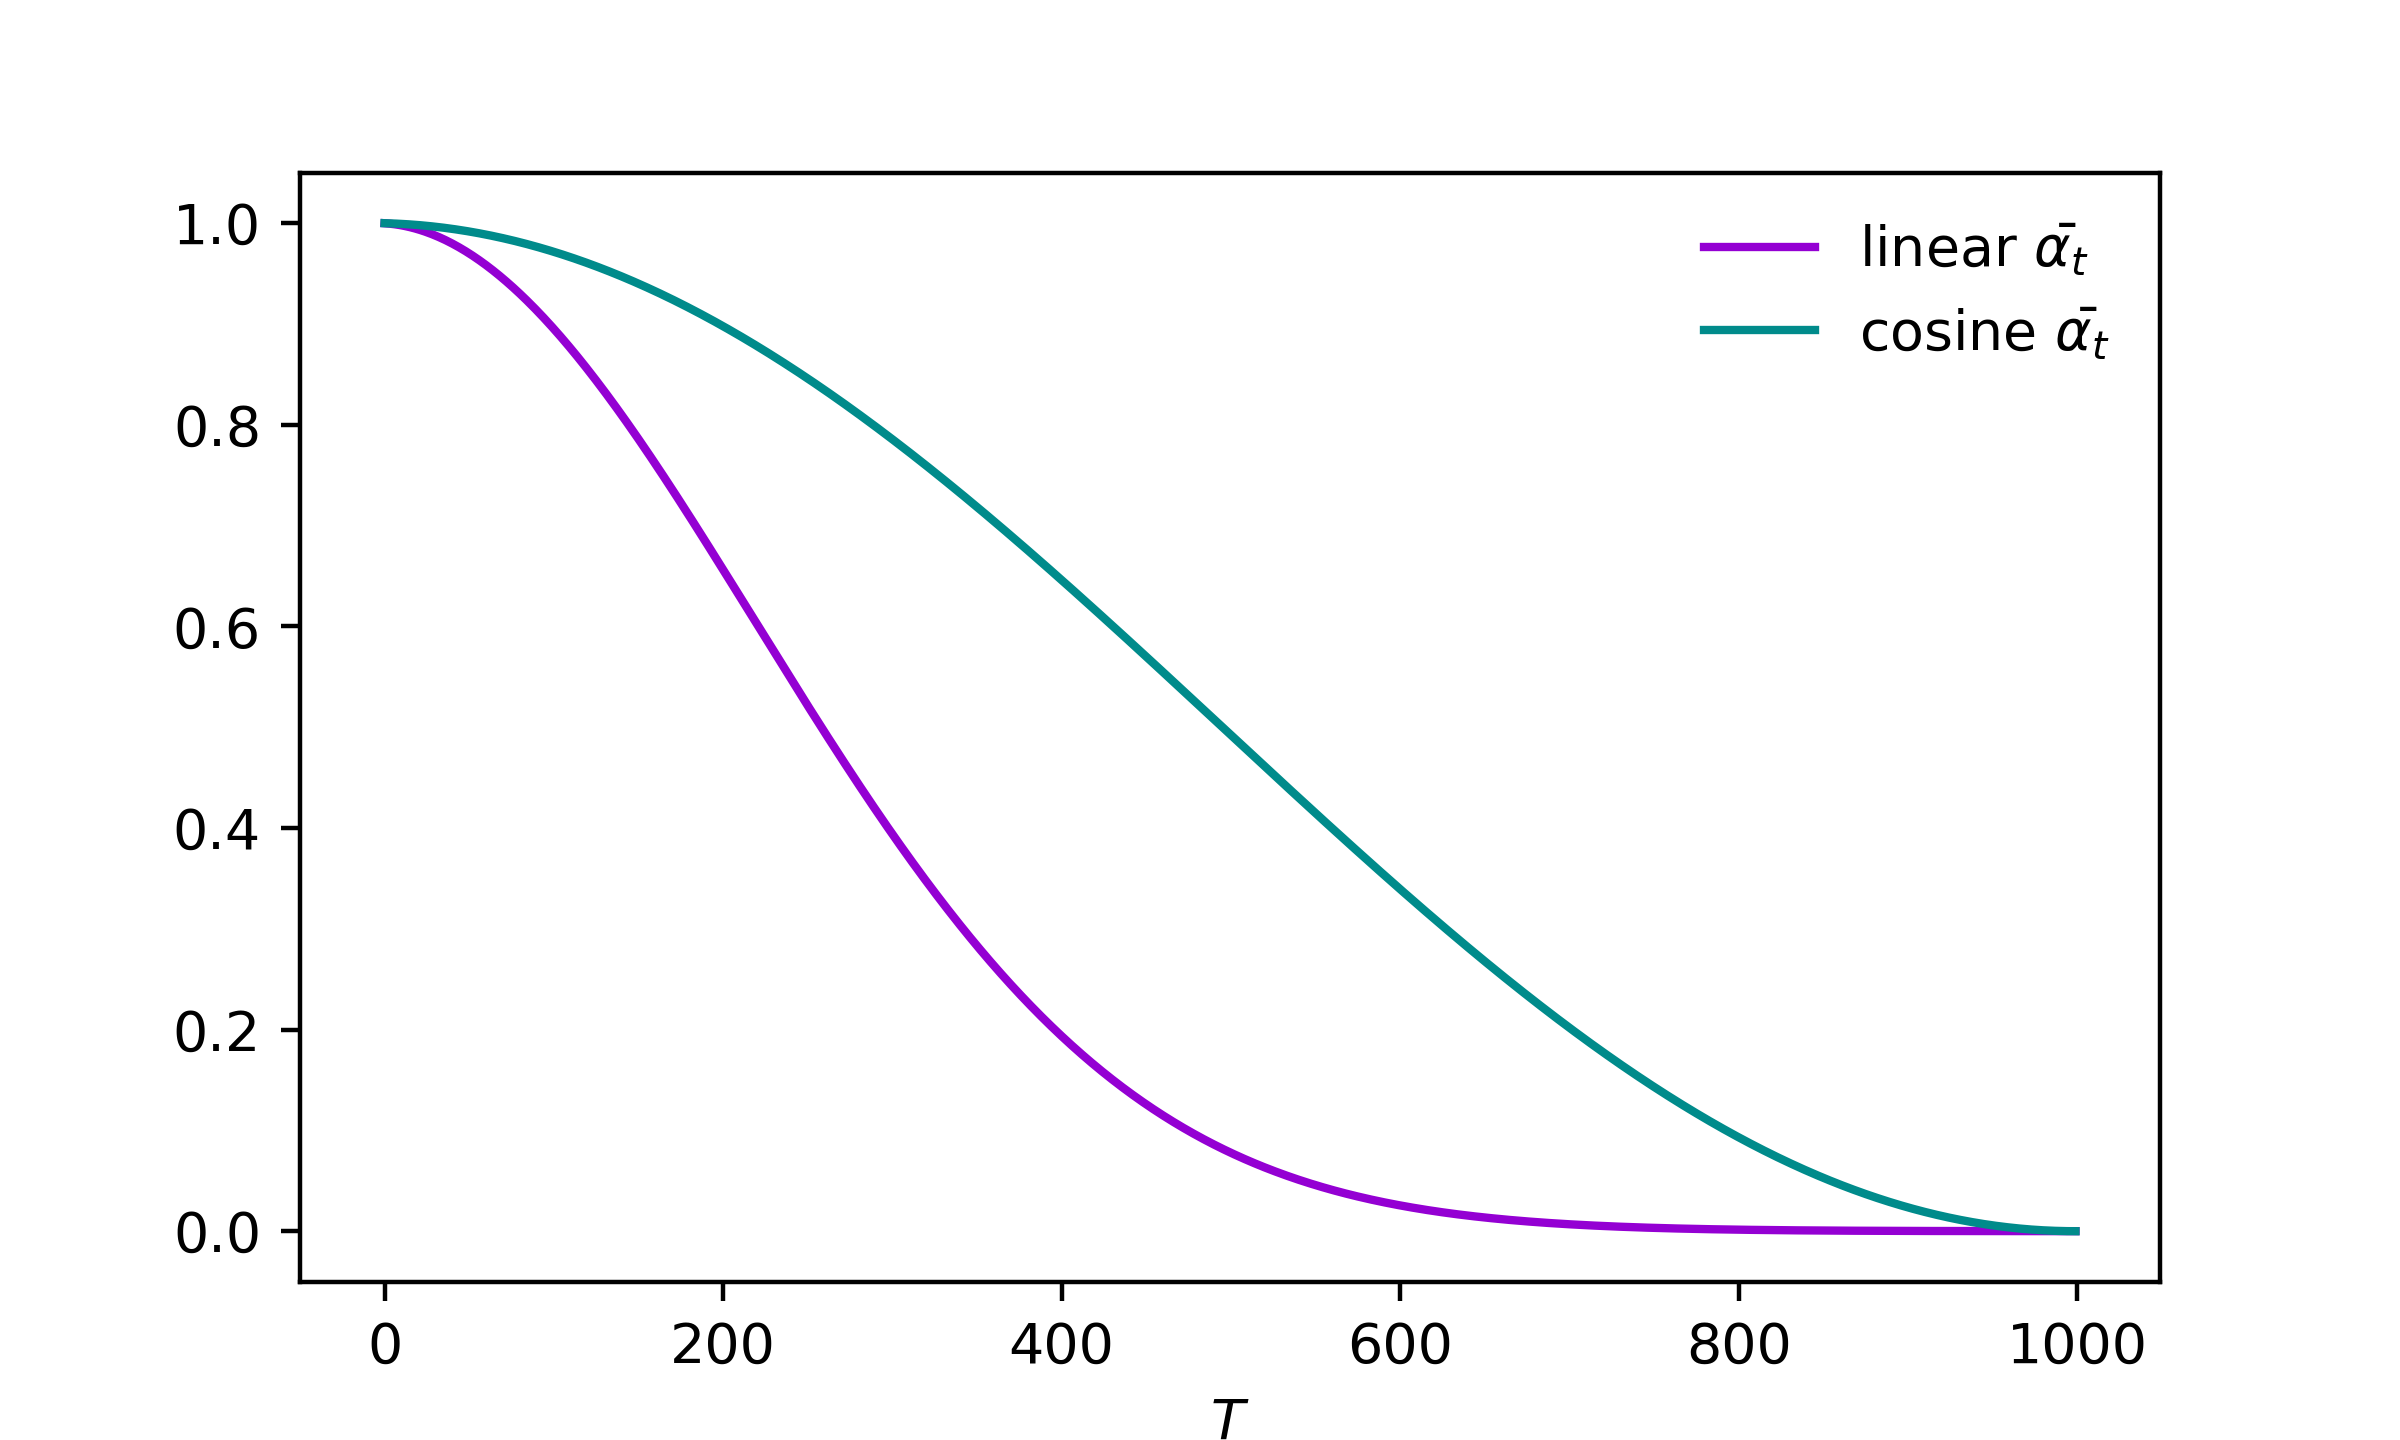
\includegraphics[scale=0.75]{ch2-diffusion-models/ddpm-linear-cosine-scheduler.png}
    \captionsetup{width=\textwidth} % set the width of the caption
    \caption{\textbf{Linear vs. Cosine scheduler} introduce in \cite{nichol2021improved}. Destroying the input structure smoothly is beneficial (regard what?) over using a simple linear scheduler \ca{esta figura suma realmente?}.}
    \label{fig:ddpm-linear-vs-cosine-scheduler}
  \end{figure}

Regarding the variance scheduler, the same work found that the linear scheduler implemented in the DDPM paper was suboptimal because destroying the image very early in the backward chain left a lot of intermediate states redundant. Instead, a cosine scheduler was proposed, which gradually destroys the image structure, providing further informative steps to the denoiser as it shown in Figure~\ref{fig:ddpm-linear-vs-cosine-scheduler}. \\

Notably, the work of \cite{rombach2022highresolution} in improving the model architecture and the training process to scale the resolution.

\subsection{Denoising Diffusion Implicit Models}

The work of \cite{song2020denoising} introduces the Denoising Diffusion Implicit Models (DDIM) that are a score-based model that uses the denoising process to estimate the likelihood of the data. The main difference between DDIM and DDPM is that the former doesn't require a Markovian chain of states to estimate the likelihood. Instead, it uses the denoising process to estimate the likelihood of the data.\\

\begin{equation}\label{eqn:ddim-likelihood}
    x_{t-1} = 
    \sqrt{\alpha_{t-1}}\underbrace{\bigg(\frac{x_{t}-\sqrt{1-\alpha_{t}}\epsilon_{\theta}^{(t)}(x_{t})}{\sqrt{\alpha_{t}}}\bigg)}_{\text{``predicted $x_{0}$''}} 
    + \underbrace{\sqrt{1-\alpha_{t-1} - \sigma^2_{t}}~\cdot~\epsilon_{\theta}^{(t)}(x_{t})}_{\text{``direction pointing to $x_{t}$''}}
    + \underbrace{\sigma_{t}\epsilon_{t}}_{\text{random noise}}
\end{equation}

Esta subsección debe cumplir lo siguiente:

\begin{enumerate}
    \item Explicar los componentes de la ecuación de arriba.
    \item Explicar conexión de la ecuación de arriba con el modelo original DDPM.
    \item Explicar como termino sampleando en menos pasos.
    \item Crear un diagrama donde a la izquierda aparezca una imagen input, al medio el ruido estimado inicial, a la derecha la transformación con
manipulación. Basado en tutorial de Jonatthan Whitakker.
    \item Explicar la utilidad de predecir $\mathrm{x}_{0}$ con el término
    propuesto en DDIM para usarlo con clasificadores no entrenados en ruido, i.e. universal guidance.
\end{enumerate}

 In Figure~\ref{fig:ddim-inversion-pascal}...\ca{explitar experimento de Pedro Pascal para invertir la imagen..., agregará valor hacer lo mismo con SD?}

\begin{figure}[ht]
    \centering
    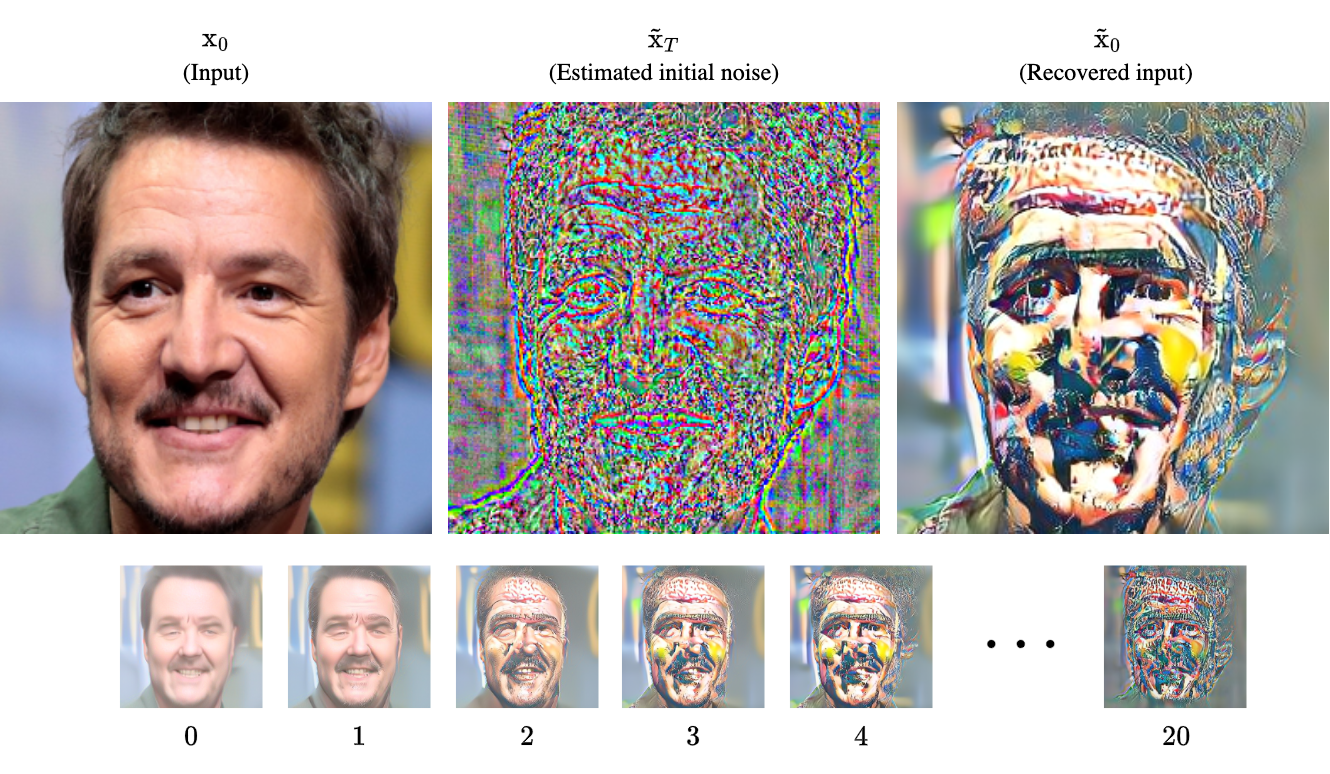
\includegraphics[scale=0.75]{ch2-diffusion-models/DDIM_Inversion_Pascal_2.png}
    \captionsetup{width=\textwidth} % set the width of the caption
    \caption{\textbf{DDIM inversion example using $50$ inference steps.} A Pedro Pascal photo to estimate the initial noise $\tilde{\mathrm{x}}_T$ using DDIM with the pretrained model \texttt{google/ddpm-celebahq-256} on the celebrity faces dataset CelebaHQ. Then, the input si reconstructed using the estimated noise as starter point. Below images are different results skpping the first $n$ inference steps of the denoising process.}
    \label{fig:ddim-inversion-pascal}
  \end{figure}

\subsection{Latent Diffusion Models}

XYZ

\section{Neural Net Architecture}

Theoretically, the model with learnable parameters used in the backward process could be anything. However, highly-dimensional data such as images, requires flexible functions that neural networks can handle properly, but not with carefully choose the proper architecture as most Deep Learning implementations. We will briefly discuss the most typical components used within the framework of diffusion models...\\

\begin{itemize}
    \item U-Net
    \item ResNet blocks
    \item Skip connections
    \item Attention blocks
    \item Adaptive group normalization (*)
    \item BigGAN residual block
\end{itemize}


\section{Summary}

In summary, a typical diffusion model framework can be implemented as follows:\\

A \textbf{forward process} that consists of a Markovian chain of states $\{\mathrm{x}\}_{0:T}$ that takes the original image $\mathrm{x}_0$ and iteratively adds noise until getting isotropic Gaussian noise $\mathrm{x}_{T}$. \\

In the reverse, or \textbf{backward process}, a model learns how to gradually remove the noise to recover the data structure. Most implementations model this denoising endeavour using some U-net neural network architecture with attention modules. \\

The sequence of intermediate states provides a detailed roadmap when destroying the observation such as images and leaves a trail to the denoiser network to recover the input structure. Therefore, the forward process acts in a \textbf{self-supervised} manner generating the labels for the data itself. \\

It is possible to use a model to predict the noisy image directly, or indirectly via predicting the noise, and then substracting from the state. Nevertheless, \textbf{the core idea of the training objective is to reduce the error between the noise prediction and the true noise} used to destroy the sample at a given step. \\

The noise used to destroy the structure in data is carefully handled by a deterministic function called \textbf{noise scheduler}. It determines the variance schedule, $\beta_{1}, \dots, \beta_{T}$, or the specific amount of noise injected in each timestamp $t$ during the Markovian chain. \\

Finally, we have a model that can \textbf{generate novel samples} from the data distribution \textbf{by sampling from a standard normal distribution and then 
successively remove noise}.
